%package list
\documentclass{article}
\usepackage[top=3cm, bottom=3cm, outer=3cm, inner=3cm]{geometry}
\usepackage{multicol}
\usepackage{graphicx}
\usepackage{url}
%\usepackage{cite}
\usepackage{hyperref}
\usepackage{array}
%\usepackage{multicol}
\newcolumntype{x}[1]{>{\centering\arraybackslash\hspace{0pt}}p{#1}}
\usepackage{natbib}
\usepackage{pdfpages}
\usepackage{multirow}
\usepackage[normalem]{ulem}
\useunder{\uline}{\ul}{}
\usepackage{svg}
\usepackage{xcolor}
\usepackage{listings}
\lstdefinestyle{ascii-tree}{
    literate={├}{|}1 {─}{--}1 {└}{+}1 
  }
\lstset{basicstyle=\ttfamily,
  showstringspaces=false,
  commentstyle=\color{red},
  keywordstyle=\color{blue}
}
%\usepackage{booktabs}
\usepackage{caption}
\usepackage{subcaption}
\usepackage{float}
\usepackage{array}

\newcolumntype{M}[1]{>{\centering\arraybackslash}m{#1}}
\newcolumntype{N}{@{}m{0pt}@{}}


%%%%%%%%%%%%%%%%%%%%%%%%%%%%%%%%%%%%%%%%%%%%%%%%%%%%%%%%%%%%%%%%%%%%%%%%%%%%
%%%%%%%%%%%%%%%%%%%%%%%%%%%%%%%%%%%%%%%%%%%%%%%%%%%%%%%%%%%%%%%%%%%%%%%%%%%%
\newcommand{\itemEmail}{aquispearr@unsa.edu.pe}

\newcommand{\itemStudentA}{Alexandra Raquel Quispe   }  

\newcommand{\itemCourse}{Programación Web II}
\newcommand{\itemCourseCode}{20231001}
\newcommand{\itemSemester}{I}
\newcommand{\itemUniversity}{Universidad Nacional de San Agustín de Arequipa}
\newcommand{\itemFaculty}{Facultad de Ingeniería de Producción y Servicios}
\newcommand{\itemDepartment}{Departamento Académico de Ingeniería de Sistemas e Informática}
\newcommand{\itemSchool}{Escuela Profesional de Ingeniería de Sistemas}
\newcommand{\itemAcademic}{2024 - A}
\newcommand{\itemInput}{Del 21 Mayo 2024}
\newcommand{\itemOutput}{Al 25 Mayo 2023}
\newcommand{\itemPracticeNumber}{05}
\newcommand{\itemTheme}{Pyton}
%%%%%%%%%%%%%%%%%%%%%%%%%%%%%%%%%%%%%%%%%%%%%%%%%%%%%%%%%%%%%%%%%%%%%%%%%%%%
%%%%%%%%%%%%%%%%%%%%%%%%%%%%%%%%%%%%%%%%%%%%%%%%%%%%%%%%%%%%%%%%%%%%%%%%%%%%

\usepackage[english,spanish]{babel}
\usepackage[utf8]{inputenc}
\AtBeginDocument{\selectlanguage{spanish}}
\renewcommand{\figurename}{Figura}
\renewcommand{\refname}{Referencias}
\renewcommand{\tablename}{Tabla} %esto no funciona cuando se usa babel
\AtBeginDocument{%
	\renewcommand\tablename{Tabla}
}

\usepackage{fancyhdr}
\pagestyle{fancy}
\fancyhf{}
\setlength{\headheight}{30pt}
\renewcommand{\headrulewidth}{1pt}
\renewcommand{\footrulewidth}{1pt}
\fancyhead[L]{\raisebox{-0.2\height}{
\includegraphics[width=3cm]{img/logo_episunsa.png}}}
\fancyhead[C]{\fontsize{7}{7}\selectfont	\itemUniversity \\ \itemFaculty \\ \itemDepartment \\ \itemSchool \\ \textbf{\itemCourse}}
\fancyhead[R]{\raisebox{-0.2\height}{
\includegraphics[width=1.2cm]{img/logo_abet}}}
\fancyfoot[L]{Quispe Arratea Alexandra}
\fancyfoot[C]{\itemCourse}
\fancyfoot[R]{Página \thepage}

% para el codigo fuente
\usepackage{listings}
\usepackage{color, colortbl}
\definecolor{dkgreen}{rgb}{0,0.6,0}
\definecolor{gray}{rgb}{0.5,0.5,0.5}
\definecolor{mauve}{rgb}{0.58,0,0.82}
\definecolor{codebackground}{rgb}{0.95, 0.95, 0.92}
\definecolor{tablebackground}{rgb}{0.8, 0, 0}

\lstset{frame=tb,
	language=bash,
	aboveskip=3mm,
	belowskip=3mm,
	showstringspaces=false,
	columns=flexible,
	basicstyle={\small\ttfamily},
	numbers=none,
	numberstyle=\tiny\color{gray},
	keywordstyle=\color{blue},
	commentstyle=\color{dkgreen},
	stringstyle=\color{mauve},
	breaklines=true,
	breakatwhitespace=true,
	tabsize=3,
	backgroundcolor= \color{codebackground},
}

\begin{document}
	
	\vspace*{10px}
	
	\begin{center}	
		\fontsize{17}{17} \textbf{ Informe de Laboratorio \itemPracticeNumber}
	\end{center}
	\centerline{\textbf{\Large Tema: \itemTheme}}
	%\vspace*{0.5cm}	

	\begin{flushright}
		\begin{tabular}{|M{2.5cm}|N|}
			\hline 
			\rowcolor{tablebackground}
			\color{white} \textbf{Nota}  \\
			\hline 
			     \\[30pt]
			\hline 			
		\end{tabular}
	\end{flushright}	

	\begin{table}[H]
		\begin{tabular}{|x{4.7cm}|x{4.8cm}|x{4.8cm}|}
			\hline 
			\rowcolor{tablebackground}
			\color{white} \textbf{Estudiante} & \color{white}\textbf{Escuela}  & \color{white}\textbf{Asignatura}   \\
			\hline 
			{\itemStudentA 
   \itemStudentB
   \itemStudentC 
   \par } & \itemSchool & {\itemCourse \par Semestre: \itemSemester \par Código: \itemCourseCode}     \\
			\hline 			
		\end{tabular}
	\end{table}		
	
	\begin{table}[H]
		\begin{tabular}{|x{4.7cm}|x{4.8cm}|x{4.8cm}|}
			\hline 
			\rowcolor{tablebackground}
			\color{white}\textbf{Laboratorio} & \color{white}\textbf{Tema}  & \color{white}\textbf{Duración}   \\
			\hline 
			\itemPracticeNumber & \itemTheme & 12 horas   \\
			\hline 
		\end{tabular}
	\end{table}
	
	\begin{table}[H]
		\begin{tabular}{|x{4.7cm}|x{4.8cm}|x{4.8cm}|}
			\hline 
			\rowcolor{tablebackground}
			\color{white}\textbf{Semestre académico} & \color{white}\textbf{Fecha de inicio}  & \color{white}\textbf{Fecha de entrega}   \\
			\hline 
			\itemAcademic & \itemInput &  \itemOutput  \\
			\hline 
		\end{tabular}
	\end{table}
	
\section{Ejercicios Propuestos}

En esta tarea, individualmente usted pondrá en práctica sus conocimientos de programación en Python para dibujar un tablero de Ajedrez. La parte gráfica ya está programada, usted sólo tendrá que concentrarse en las estructuras de datos subyacentes. Con el código proporcionado usted dispondrá de varios objetos de tipo \texttt{Picture} para poder realizar su tarea:

\begin{itemize}
    \item \texttt{rock}
    \item \texttt{knight}
    \item \texttt{bishop}
    \item \texttt{queen}
    \item \texttt{king}
    \item \texttt{square}
\end{itemize}

Estos objetos estarán disponibles importando la biblioteca: \texttt{chessPictures} y estarán internamente representados con arreglos de strings que podrá revisar en el archivo \texttt{pieces.py}.

La clase \texttt{Picture} tiene un sólo atributo: el arreglo de strings \texttt{img}, el cual contendrá la representación en caracteres de la figura que se desea dibujar. La clase \texttt{Picture} ya cuenta con una función implementada, no debe modificarla, pero si puede usarla para implementar sus otras funciones:
\begin{itemize}
    \item \texttt{\_invColor}: recibe un color como un carácter de texto y devuelve su color negativo, también como texto, deberá revisar el archivo \texttt{colors.py} para conocer los valores negativos de cada carácter.
\end{itemize}

La clase \texttt{Picture} contará además con varios métodos que usted deberá implementar:
\begin{itemize}
    \item \texttt{verticalMirror}: Devuelve el espejo vertical de la imagen
    \item \texttt{horizontalMirror}: Devuelve el espejo horizontal de la imagen
    \item \texttt{negative}: Devuelve un negativo de la imagen
    \item \texttt{join}: Devuelve una nueva figura poniendo la figura del argumento al lado derecho de la figura actual
    \item \texttt{up}: Devuelve una nueva figura poniendo la figura recibida como argumento, encima de la figura actual
    \item \texttt{under}: Devuelve una nueva figura poniendo la figura recibida como argumento, sobre la figura actual
    \item \texttt{horizontalRepeat}: Devuelve una nueva figura repitiendo la figura actual al costado la cantidad de veces que indique el valor de \texttt{n}
    \item \texttt{verticalRepeat}: Devuelve una nueva figura repitiendo la figura actual debajo, la cantidad de veces que indique el valor de \texttt{n}
\end{itemize}

Tenga en cuenta que para implementar todos estos métodos, sólo deberá trabajar sobre la representación interna de un \texttt{Picture}, es decir su atributo \texttt{img}.

Para dibujar una objeto \texttt{Picture} bastará importar el método \texttt{draw} de la biblioteca \texttt{interpreter} y usarlo de la siguiente manera:

\begin{verbatim}
>>> from chessPictures import *
>>> from interpreter import draw
>>> draw(rock)
\end{verbatim}

Considere el repositorio:
\url{https://github.com/rescobedoq/pw2/tree/main/labs/lab04/Tarea-del-Ajedrez}

\section{Ejercicios}
Para resolver los siguientes ejercicios sólo está permitido usar ciclos, condicionales, definición de listas por comprensión, sublistas, \texttt{map}, \texttt{join}, \texttt{+}, \texttt{lambda}, \texttt{zip}, \texttt{append}, \texttt{pop}, \texttt{range}. Implemente los métodos de la clase \texttt{Picture}. Se recomienda que implemente la clase \texttt{Picture} por etapas, probando realizar los dibujos que se muestran en las siguientes preguntas. Usando únicamente los métodos de los objetos de la clase \texttt{Picture}, dibuje las siguientes figuras (invoque a \texttt{draw}):

		
\section{Equipos, materiales y temas utilizados}
\begin{itemize}
    \item \textbf{Sistema Operativo:} Ubuntu GNU/Linux 23.04 Lunar Lobster 64 bits, Kernel 6.2.
    \item \textbf{Editor de texto:} VIM 9.0.
    \item \textbf{Entorno de desarrollo:} Python 3.10.
    \item \textbf{Control de versiones:} Git 2.39.2.
    \item \textbf{Repositorio:} Cuenta en GitHub con el correo institucional.
    \item \textbf{Bibliotecas utilizadas:}
    \begin{itemize}
        \item \textbf{chessPictures:} Para el manejo y representación gráfica de piezas de ajedrez.
        \item \textbf{interpreter:} Para dibujar los objetos de tipo \texttt{Picture}.
    \end{itemize}
    \item \textbf{Tecnologías y métodos utilizados:}
    \begin{itemize}
        \item \textbf{Python:} Utilizado para implementar las estructuras de datos y métodos necesarios para manipular y visualizar las piezas de ajedrez.
        \item \textbf{GitHub:} Para la gestión y control de versiones del código fuente del proyecto.
    \end{itemize}
\end{itemize}


\section{URL de Repositorio GitHub}
\begin{itemize}
    \item URL del Repositorio GitHub para clonar o recuperar.
    \item \url{https://github.com/aquispearr/Pweb2_Lab05.git}
    \item URL deL video explicativo.
    \item \url{https://docs.google.com/document/d/1eUpm0Yp-VVFlS1BXQTqXK0amFvjJQZWHBrFFK2JonhY/edit?usp=sharing}
\end{itemize}

\section{Actividades con el repositorio GitHub}

\subsection{Implementación de la clase \texttt{Picture}}

En esta sección se explica la implementación de la clase \texttt{Picture} que permite manipular y dibujar figuras representadas por arreglos de strings. A continuación, se detallan las funciones y métodos de la clase.

\begin{itemize}
    \item \textbf{Definición e inicialización de la clase}

\lstinputlisting[language=Python, caption={Definición e inicialización de la clase \texttt{Picture}}, label={lst:inicializacion}]{initialization.py}

\textbf{Explicación:}
\begin{itemize}
    \item \texttt{\_\_init\_\_}: Este método es el constructor de la clase \texttt{Picture}, que inicializa un objeto \texttt{Picture} con el atributo \texttt{img}, que es una lista de strings que representa la imagen.
    \item \texttt{\_\_eq\_\_}: Este método permite comparar dos objetos \texttt{Picture} para verificar si son iguales, basándose en su atributo \texttt{img}.
    \item \texttt{\_invColor}: Este método privado invierte el color de un carácter utilizando un diccionario de colores invertidos.
\end{itemize}

    \item \textbf{Método \texttt{verticalMirror}}

\lstinputlisting[language=Python, caption={Método \texttt{verticalMirror}}, label={lst:verticalMirror}]{vertical_mirror.py}

\textbf{Explicación:}
Este método devuelve un nuevo objeto \texttt{Picture} cuya imagen es el espejo vertical de la imagen original. Para lograrlo, se invierte cada string de la lista \texttt{img} utilizando el slicing de Python \texttt{[::-1]}.

    \item \textbf{Método \texttt{horizontalMirror}}

\lstinputlisting[language=Python, caption={Método \texttt{horizontalMirror}}, label={lst:horizontalMirror}]{horizontal_mirror.py}

\textbf{Explicación:}
Este método devuelve un nuevo objeto \texttt{Picture} cuya imagen es el espejo horizontal de la imagen original. Para ello, se invierte la lista \texttt{img} utilizando el slicing de Python \texttt{[::-1]}.

    \item \textbf{Método \texttt{negative}}

\lstinputlisting[language=Python, caption={Método \texttt{negative}}, label={lst:negative}]{negative.py}

\textbf{Explicación:}
Este método devuelve un nuevo objeto \texttt{Picture} cuya imagen es el negativo de la imagen original. Para lograrlo, se itera sobre cada fila de la imagen (\texttt{self.img}) y se crea una nueva fila invirtiendo el color de cada carácter utilizando el método \texttt{\_invColor}. Todas las filas invertidas se almacenan en una nueva lista llamada \texttt{negativo}, y luego se crea una nueva instancia de \texttt{Picture} con esta lista de filas invertidas.

    \item \textbf{Método \texttt{join}}

\lstinputlisting[language=Python, caption={Método \texttt{join}}, label={lst:join}]{join.py}

\textbf{Explicación:}
Este método devuelve un nuevo objeto \texttt{Picture} cuya imagen es la concatenación horizontal de la imagen actual con la imagen del objeto \texttt{Picture} pasado como argumento. Se itera sobre los índices de las filas y se concatenan las filas correspondientes de \texttt{self.img} y \texttt{p.img}. Las filas concatenadas se almacenan en una nueva lista llamada \texttt{unido}, y se crea una nueva instancia de \texttt{Picture} con esta lista de filas unidas.

    \item \textbf{Método \texttt{up}}

\lstinputlisting[language=Python, caption={Método \texttt{up}}, label={lst:up}]{up.py}

\textbf{Explicación:}
Este método devuelve un nuevo objeto \texttt{Picture} cuya imagen es la concatenación vertical de la imagen actual con la imagen del objeto \texttt{Picture} pasado como argumento. Se crea una nueva lista llamada \texttt{compuesto} que contiene todas las filas de \texttt{self.img} seguidas de todas las filas de \texttt{p.img}. Esta lista se utiliza para crear una nueva instancia de \texttt{Picture} que representa la imagen compuesta.

    \item \textbf{Método \texttt{under}}

\lstinputlisting[language=Python, caption={Método \texttt{under}}, label={lst:under}]{under.py}

\textbf{Explicación:}
Este método devuelve un nuevo objeto \texttt{Picture} cuya imagen es la superposición de la imagen del objeto \texttt{Picture} pasado como argumento sobre la imagen actual. Se itera sobre las filas y columnas de \texttt{p.img} y, si un carácter en \texttt{p.img} es un espacio en blanco, se reemplaza por el carácter correspondiente de \texttt{self.img}. Las filas superpuestas se almacenan en una nueva lista llamada \texttt{sobrepuesto}, y se crea una nueva instancia de \texttt{Picture} con esta lista.

    \item \textbf{Método \texttt{horizontalRepeat}}

\lstinputlisting[language=Python, caption={Método \texttt{horizontalRepeat}}, label={lst:horizontalRepeat}]{horizontal_repeat.py}

\textbf{Explicación:}
Este método devuelve un nuevo objeto \texttt{Picture} cuya imagen es la repetición horizontal de la imagen actual \texttt{n} veces. Se itera sobre cada fila de \texttt{self.img} y se crea una nueva fila repitiendo esa fila \texttt{n} veces utilizando la multiplicación de cadenas (\texttt{fila * n}). Las filas repetidas se almacenan en una nueva lista llamada \texttt{repetidoH}, y se crea una nueva instancia de \texttt{Picture} con esta lista.

    \item \textbf{Método \texttt{verticalRepeat}}

\lstinputlisting[language=Python, caption={Método \texttt{verticalRepeat}}, label={lst:verticalRepeat}]{vertical_repeat.py}

\textbf{Explicación:}
Este método devuelve un nuevo objeto \texttt{Picture} cuya imagen es la repetición vertical de la imagen actual \texttt{n} veces. Se crea una nueva lista llamada \texttt{repetidoV} que contiene todas las filas de \texttt{self.img} repetidas \texttt{n} veces. Esta lista se utiliza para crear una nueva instancia de \texttt{Picture} que representa la imagen repetida verticalmente.

    \item \textbf{Método \texttt{rotate}}

\lstinputlisting[language=Python, caption={Método \texttt{rotate}}, label={lst:rotate}]{rotate.py}

\textbf{Explicación:}
Este método devuelve un nuevo objeto \texttt{Picture} cuya imagen es la rotación de 90 grados en sentido antihorario de la imagen original. Se crea una nueva lista llamada \texttt{b} que almacenará las filas de la imagen rotada. Se itera sobre los índices de las columnas de la imagen original y, para cada índice \texttt{i}, se crea una nueva cadena \texttt{a} que contiene los caracteres de la columna \texttt{i} de la imagen original, pero en orden inverso (comenzando desde la parte inferior de la columna). Cada cadena \texttt{a} se agrega a la lista \text



\subsection{Ejercicios propuestos}

\subsubsection{Ejercicio 2A}

\begin{lstlisting}[language=Python, caption={Código del ejercicio 2A}]
from interpreter import draw
from chessPictures import *

caballo1 = Picture(KNIGHT)
caballo2 = caballo1.negative()
fila1 = caballo1.join(caballo2)
fila2 = fila1.negative()
tablero = fila1.up(fila2)
draw(tablero)
\end{lstlisting}

\textbf{Explicación:}
\begin{itemize}
    \item Se importan los módulos necesarios: \texttt{interpreter} para la función \texttt{draw} y \texttt{chessPictures} para acceder a la representación del caballo de ajedrez (\texttt{KNIGHT}).
    \item Se crea un objeto \texttt{Picture} \texttt{caballo1} a partir de la representación del caballo de ajedrez.
    \item Se crea un objeto \texttt{Picture} \texttt{caballo2} que es el negativo de \texttt{caballo1}.
    \item Se concatena horizontalmente \texttt{caballo1} y \texttt{caballo2} para formar la \texttt{fila1}.
    \item Se crea \texttt{fila2} como el negativo de \texttt{fila1}.
    \item Se concatena verticalmente \texttt{fila1} y \texttt{fila2} para formar el \texttt{tablero}.
    \item Finalmente, se utiliza la función \texttt{draw} para dibujar el \texttt{tablero}.
\end{itemize}

\textbf{Resultado:}
El resultado de este código es un tablero de ajedrez formado por caballos blancos y negros, como se muestra en la siguiente imagen:

\begin{figure}[H]
    \centering
    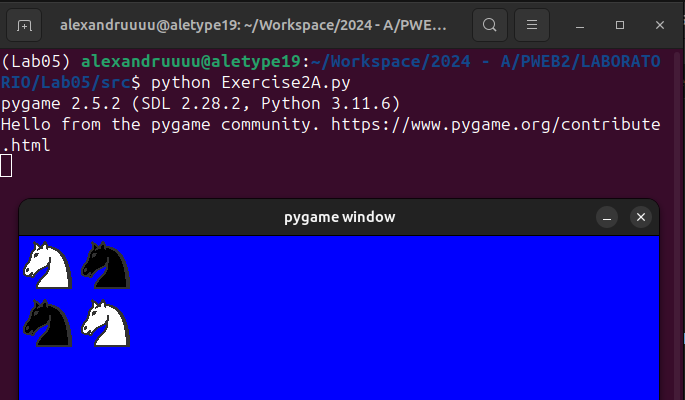
\includegraphics[width=0.8\textwidth]{img/1.png}
    \caption{Resultado del ejercicio 2A}
    \label{fig:ejercicio2a}
\end{figure}

\subsubsection{Ejercicio 2B}

\begin{lstlisting}[language=Python, caption={Código del ejercicio 2B}]
from interpreter import draw
from chessPictures import *

caballo1 = Picture(KNIGHT)
caballo2 = caballo1.negative()
fila1 = caballo1.join(caballo2)
fila2 = fila1.verticalMirror()
tablero = fila1.up(fila2)
draw(tablero)
\end{lstlisting}

\textbf{Explicación:}
\begin{itemize}
    \item Se importan los módulos necesarios: \texttt{interpreter} para la función \texttt{draw} y \texttt{chessPictures} para acceder a la representación del caballo de ajedrez (\texttt{KNIGHT}).
    \item Se crea un objeto \texttt{Picture} \texttt{caballo1} a partir de la representación del caballo de ajedrez.
    \item Se crea un objeto \texttt{Picture} \texttt{caballo2} que es el negativo de \texttt{caballo1}.
    \item Se concatena horizontalmente \texttt{caballo1} y \texttt{caballo2} para formar la \texttt{fila1}.
    \item Se crea \texttt{fila2} como el espejo vertical de \texttt{fila1} utilizando el método \texttt{verticalMirror}.
    \item Se concatena verticalmente \texttt{fila1} y \texttt{fila2} para formar el \texttt{tablero}.
    \item Finalmente, se utiliza la función \texttt{draw} para dibujar el \texttt{tablero}.
\end{itemize}

\textbf{Resultado:}
El resultado de este código es un tablero de ajedrez formado por caballos blancos y negros, donde la mitad inferior es el espejo vertical de la mitad superior, como se muestra en la siguiente imagen:

\begin{figure}[H]
    \centering
    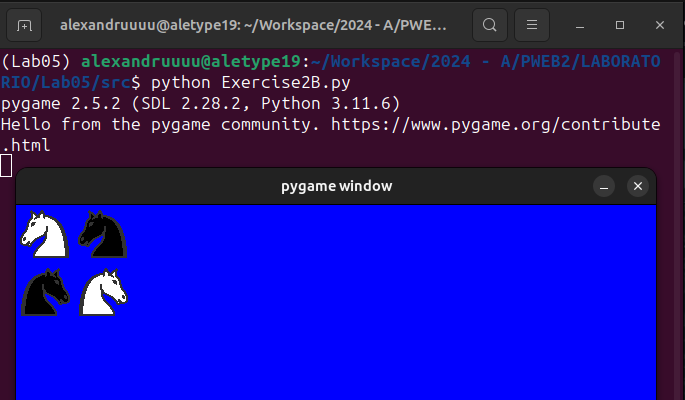
\includegraphics[width=0.8\textwidth]{img/2.png}
    \caption{Resultado del ejercicio 2B}
    \label{fig:ejercicio2b}
\end{figure}



\subsubsection{Ejercicio 2C}

\begin{lstlisting}[language=Python, caption={Código del ejercicio 2C}]
from interpreter import draw
from chessPictures import *

reyna = Picture(QUEEN)
tablero = reyna.horizontalRepeat(4)
draw(tablero)
\end{lstlisting}

\textbf{Explicación:}
\begin{itemize}
    \item Se crea un objeto \texttt{Picture} \texttt{reyna} a partir de la representación de la reina de ajedrez.
    \item Se utiliza el método \texttt{horizontalRepeat} con el argumento \texttt{4} para repetir la imagen de la reina horizontalmente cuatro veces, creando un nuevo objeto \texttt{Picture} llamado \texttt{tablero}.
    \item Finalmente, se utiliza la función \texttt{draw} para dibujar el \texttt{tablero}.
\end{itemize}

\textbf{Resultado:}
El resultado de este código es una fila con cuatro representaciones de la reina de ajedrez, como se muestra en la siguiente imagen:

\begin{figure}[H]
    \centering
    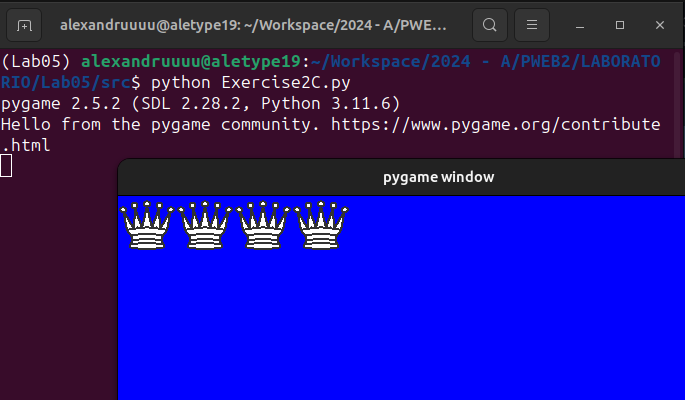
\includegraphics[width=0.8\textwidth]{img/3.png}
    \caption{Resultado del ejercicio 2C}
    \label{fig:ejercicio2c}
\end{figure}


\subsubsection{Ejercicio 2D}

\begin{lstlisting}[language=Python, caption={Código del ejercicio 2D}]
from interpreter import draw
from chessPictures import *

cuadroBlanco = Picture(SQUARE)
cuadroNegro = cuadroBlanco.negative()
tablero1 = cuadroBlanco.join(cuadroNegro)
tablero = tablero1.horizontalRepeat(4)
draw(tablero)
\end{lstlisting}

\textbf{Explicación:}
\begin{itemize}
    \item Se importan los módulos necesarios.
    \item Se crea un objeto \texttt{cuadroBlanco} a partir de la representación de un cuadro blanco (\texttt{SQUARE}).
    \item Se crea \texttt{cuadroNegro} como el negativo de \texttt{cuadroBlanco}.
    \item Se concatenan horizontalmente \texttt{cuadroBlanco} y \texttt{cuadroNegro} para formar \texttt{tablero1}.
    \item Se repite \texttt{tablero1} cuatro veces horizontalmente utilizando \texttt{horizontalRepeat} para crear \texttt{tablero}.
    \item Se dibuja \texttt{tablero} con la función \texttt{draw}.
\end{itemize}

\textbf{Resultado:}
Una fila con ocho cuadros alternando entre blanco y negro, como se muestra:

\begin{figure}[H]
    \centering
    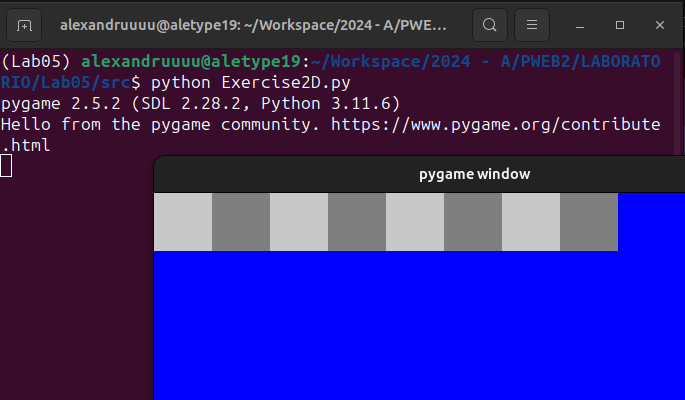
\includegraphics[width=0.75\textwidth]{img/4.png}
    \caption{Resultado del ejercicio 2D}
    \label{fig:ejercicio2d}
\end{figure}

\subsubsection{Ejercicio 2E}

\begin{lstlisting}[language=Python, caption={Código del ejercicio 2E}]
from interpreter import draw
from chessPictures import *

cuadroBlanco = Picture(SQUARE)
cuadroNegro = cuadroBlanco.negative()
tablero1 = cuadroNegro.join(cuadroBlanco)
tablero = tablero1.horizontalRepeat(4)
draw(tablero)
\end{lstlisting}

\textbf{Explicación:}
La única diferencia con el ejercicio 2D es que la concatenación horizontal de \texttt{cuadroNegro} y \texttt{cuadroBlanco} se realiza en orden inverso para formar \texttt{tablero1}.

\textbf{Resultado:}
Una fila con ocho cuadros alternando entre negro y blanco, como se muestra:

\begin{figure}[H]
    \centering
    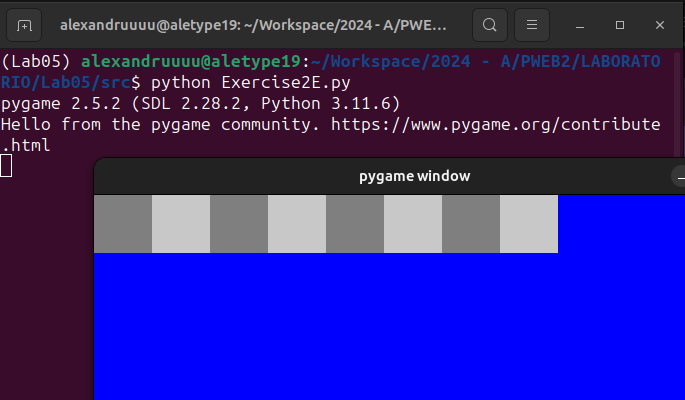
\includegraphics[width=0.8\textwidth]{img/5.png}
    \caption{Resultado del ejercicio 2E}
    \label{fig:ejercicio2e}
\end{figure}


\subsubsection{Ejercicio 2F}

\begin{lstlisting}[language=Python, caption={Código del ejercicio 2F}]
from interpreter import draw
from chessPictures import *

cuadroBlanco = Picture(SQUARE)
cuadroNegro = cuadroBlanco.negative()
tablero1 = cuadroBlanco.join(cuadroNegro).horizontalRepeat(4)
tablero2 = tablero1.negative()
tablero = tablero1.up(tablero2).verticalRepeat(2)
draw(tablero)
\end{lstlisting}

\textbf{Explicación:}
\begin{itemize}
    \item Se importan los módulos necesarios.
    \item Se crea un objeto \texttt{cuadroBlanco} a partir de la representación de un cuadro blanco (\texttt{SQUARE}).
    \item Se crea \texttt{cuadroNegro} como el negativo de \texttt{cuadroBlanco}.
    \item Se concatenan horizontalmente \texttt{cuadroBlanco} y \texttt{cuadroNegro}, y luego se repite este patrón cuatro veces horizontalmente para formar \texttt{tablero1}.
    \item Se crea \texttt{tablero2} como el negativo de \texttt{tablero1}.
    \item Se concatenan verticalmente \texttt{tablero1} y \texttt{tablero2} para formar una fila completa, y luego se repite este patrón dos veces verticalmente para formar \texttt{tablero}.
    \item Se dibuja \texttt{tablero} con la función \texttt{draw}.
\end{itemize}

\textbf{Resultado:}
Un tablero de ajedrez completo de 8x8 cuadros alternando entre blanco y negro, como se muestra:

\begin{figure}[H]
    \centering
    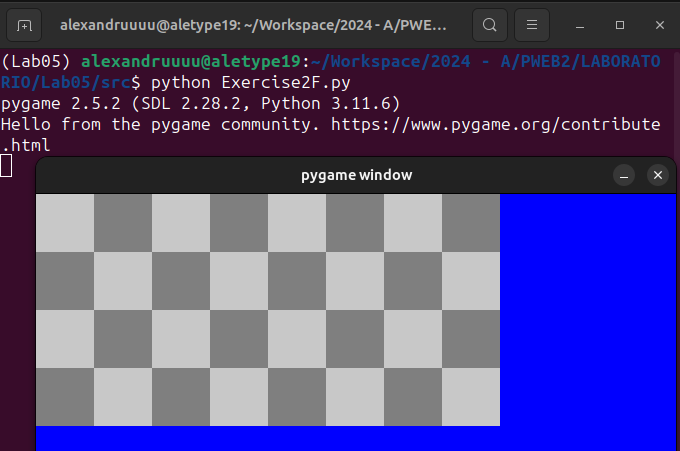
\includegraphics[width=0.8\textwidth]{img/6.png}
    \caption{Resultado del ejercicio 2F}
    \label{fig:ejercicio2f}
\end{figure}

\subsubsection{Ejercicio Final}

\begin{lstlisting}[language=Python, caption={Código del ejercicio final}]
from interpreter import draw
from chessPictures import *

cuadroBlanco = Picture(SQUARE)
cuadroNegro = cuadroBlanco.negative()
tablero1 = cuadroBlanco.join(cuadroNegro).horizontalRepeat(4)
tablero2 = tablero1.negative()
fila1 = rock.join(knight).join(bishop).join(queen).join(king).join(bishop).join(knight).join(rock)
fila2 = pawn.horizontalRepeat(8)
tableroSuperior = tablero2.up(tablero1).under(fila1.up(fila2)).negative()
tableroMedio = tablero1.up(tablero2).verticalRepeat(2)
tableroInferior = tablero1.up(tablero2).under(fila2.up(fila1))
final = tableroSuperior.up(tableroMedio).up(tableroInferior)
draw(final)
\end{lstlisting}

\textbf{Explicación:}
Este código crea un tablero de ajedrez completo con todas las piezas en sus posiciones iniciales. Primero, se construyen las filas de cuadros blancos y negros utilizando los métodos \texttt{join} y \texttt{horizontalRepeat}. Luego, se crean las filas con las piezas de ajedrez, utilizando las representaciones importadas desde el módulo \texttt{chessPictures}.

A continuación, se construyen tres secciones principales del tablero: la sección superior con las piezas blancas, la sección media con cuadros vacíos y la sección inferior con las piezas negras. Cada sección se crea combinando las filas de cuadros y piezas mediante los métodos \texttt{up}, \texttt{under} y \texttt{verticalRepeat}.

Finalmente, se ensambla el tablero completo concatenando verticalmente las tres secciones principales utilizando el método \texttt{up}. El resultado final se dibuja con la función \texttt{draw}.

\textbf{Resultado:}
Un tablero de ajedrez completo con todas las piezas en sus posiciones iniciales, como se muestra en la siguiente imagen:

\begin{figure}[H]
    \centering
    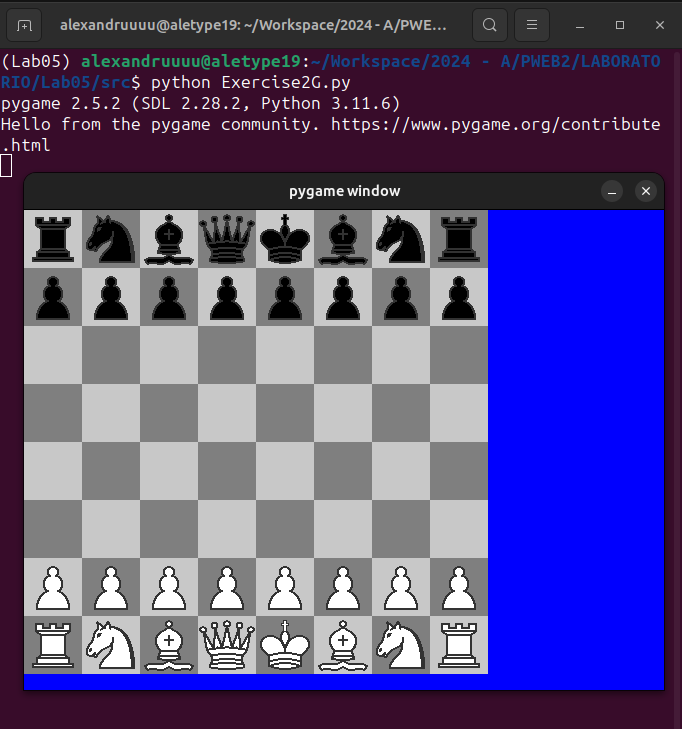
\includegraphics[width=0.8\textwidth]{img/7.png}
    \caption{Resultado del ejercicio final}
    \label{fig:ejerciciofinal}
\end{figure}



%%%%%%%%%%%%%%%%%%%%%%%%%%%%%%%%%%%%%%%%%%%%%%%%%%%%%%%%%%%%%%%%%%%%%%%%%%%%%%%%%%%%%%%%%%%%%%%%%%%%%%%%%
%%%%%%%%%%%%%%%%%%%%%%%%%%%%%%%%%%%		


\section{Rubrica}	
\subsection{\textcolor{red}{Rúbrica para el contenido del Informe y demostración}}
	\begin{itemize}			
		\item El alumno debe marcar o dejar en blanco en celdas de la columna \textbf{Checklist} si cumplio con el ítem correspondiente.
		\item Si un alumno supera la fecha de entrega,  su calificación será sobre la nota mínima aprobada, siempre y cuando cumpla con todos lo items.
		\item El alumno debe autocalificarse en la columna \textbf{Estudiante} de acuerdo a la siguiente tabla:
	
		\begin{table}[ht]
			\caption{Niveles de desempeño}
			\begin{center}
			\begin{tabular}{ccccc}
    			\hline
    			 & \multicolumn{4}{c}{Nivel}\\
    			\cline{1-5}
    			\textbf{Puntos} & Insatisfactorio 25\%& En Proceso 50\% & Satisfactorio 75\% & Sobresaliente 100\%\\
    			\textbf{2.0}&0.5&1.0&1.5&2.0\\
    			\textbf{4.0}&1.0&2.0&3.0&4.0\\
    		\hline
			\end{tabular}
		\end{center}
	\end{table}	
	
	\end{itemize}
	
	\begin{table}[H]
		\caption{Rúbrica para contenido del Informe y demostración}
		\setlength{\tabcolsep}{0.5em} % for the horizontal padding
		{\renewcommand{\arraystretch}{1.5}% for the vertical padding
		%\begin{center}
		\begin{tabular}{|p{2.7cm}|p{7cm}|x{1.3cm}|p{1.2cm}|p{1.5cm}|p{1.1cm}|}
			\hline
    		\multicolumn{2}{|c|}{Contenido y demostración} & Puntos & Checklist & Estudiante & Profesor\\
			\hline
			\textbf{1. GitHub} & Hay enlace URL activo del directorio para el  laboratorio hacia su repositorio GitHub con código fuente terminado y fácil de revisar. &2 &X &2 & \\ 
			\hline
			\textbf{2. Commits} &  Hay capturas de pantalla de los commits más importantes con sus explicaciones detalladas. (El profesor puede preguntar para refrendar calificación). &4 &X &2 &  \\ 
			\hline 
			\textbf{3. Código fuente} &  Hay porciones de código fuente importantes con numeración y explicaciones detalladas de sus funciones. &2 &X &1 & \\ 
			\hline 
			\textbf{4. Ejecución} & Se incluyen ejecuciones/pruebas del código fuente  explicadas gradualmente. &2 &X &1 & \\ 
			\hline			
			\textbf{5. Pregunta} & Se responde con completitud a la pregunta formulada en la tarea.  (El profesor puede preguntar para refrendar calificación).  &2 &X &2 & \\ 
			\hline	
			\textbf{6. Fechas} & Las fechas de modificación del código fuente estan dentro de los plazos de fecha de entrega establecidos. &2 &X &2 & \\ 
			\hline 
			\textbf{7. Ortografía} & El documento no muestra errores ortográficos. &2 &X &2 & \\ 
			\hline 
			\textbf{8. Madurez} & El Informe muestra de manera general una evolución de la madurez del código fuente,  explicaciones puntuales pero precisas y un acabado impecable.   (El profesor puede preguntar para refrendar calificación).  &4 &X &3 & \\ 
			\hline
			\multicolumn{2}{|c|}{\textbf{Total}} &20 & &15 & \\ 
			\hline
		\end{tabular}
		%\end{center}
		%\label{tab:multicol}
		}
	\end{table}
	
\clearpage



	
%\clearpage
%\bibliographystyle{apalike}
%\bibliographystyle{IEEEtranN}
%\bibliography{bibliography}
			
\end{document}